\documentclass[12pt, a4paper, oneside]{ctexart}
\usepackage{amsmath, amsthm, amssymb, bm, color, graphicx, geometry, hyperref, mathrsfs,extarrows, braket, booktabs, array}
\setmainfont{Times New Roman}  % 设置英文字体
\setsansfont{Calibri}
\setmonofont{Consolas}

\linespread{1.4}
%\geometry{left=2.54cm,right=2.54cm,top=3.18cm,bottom=3.18cm}
\geometry{left=1.84cm,right=1.84cm,top=2.18cm,bottom=2.18cm}
\newenvironment{problem}{\par\noindent\textbf{题目. }}{\bigskip\par}
\newenvironment{solution}{\par\noindent\textbf{解答. }}{\bigskip\par}
\newenvironment{note}{\par\noindent\textbf{注记. }}{\bigskip\par}

\everymath{\displaystyle} % 默认全部行间公式
\DeclareMathOperator*\uplim{\overline{lim}} % 定义上极限 \uplim_{}
\DeclareMathOperator*\lowlim{\underline{lim}} % 定义下极限 \lowlim_{}
\let\leq=\leqslant % 将全部leq变为leqslant
\let\geq=\geqslant % geq同理

% 一些宏定义
\def\bd{\boldsymbol}    % 加粗(向量) boldsymbol
\def\disp{\displaystyle}% 使用行间公式 displaystyle(默认)
\def\tsty{\textstyle}   % 使用行内公式 textstyle
\def\sign{\text{sign}}  % sign function
\def\wtd{\widetilde}    % 宽波浪线 widetilde
\def\R{\mathbb{R}}      % Real number
\def\Q{\mathbb{Q}}      % Rational number (Quotient)
\def\C{\mathbb{C}}      % Complex number
\def\d{\mathrm{d}}      % differential operator
\def\e{\mathrm{e}}      % Euler's number
\def\i{\mathrm{i}}      % imaginary number
\def\L{\mathcal{L}}     % Loss function
\def\wdh{\widehat}      % 宽帽子 widehat
\def\ol{\overline}      % 上横线 overline
\def\ul{\underline}     % 下横线 underline
\def\add{\vspace{0.5ex}}  % 增加行间距
\def\del{\vspace{-2.5ex}}  % 减少行间距

% 基本信息
\newcommand{\RQ}{\today} % 日期
\newcommand{\km}{实变函数} % 科目
\newcommand{\bj}{强基数学002} % 班级
\newcommand{\xm}{吴天阳} % 姓名
\newcommand{\xh}{2204210460} % 学号
\newcommand{\XH}{59} % 序号

\begin{document}

%\pagestyle{empty}
\pagestyle{plain}
\vspace*{-15ex}
\centerline{\begin{tabular}{*6{c}}
    \parbox[t]{0.25\linewidth}{\begin{center}\textbf{日期}\\ \large \textcolor{blue}{\RQ}\end{center}} 
    & \parbox[t]{0.15\linewidth}{\begin{center}\textbf{科目}\\ \large \textcolor{blue}{\km}\end{center}}
    & \parbox[t]{0.2\linewidth}{\begin{center}\textbf{班级}\\ \large \textcolor{blue}{\bj}\end{center}}
    & \parbox[t]{0.1\linewidth}{\begin{center}\textbf{姓名}\\ \large \textcolor{blue}{\xm}\end{center}}
    & \parbox[t]{0.15\linewidth}{\begin{center}\textbf{学号}\\ \large \textcolor{blue}{\xh}\end{center}}
    & \parbox[t]{0.1\linewidth}{\begin{center}\textbf{序号}\\ \large \textcolor{blue}{\XH}\end{center}} \\ \hline
\end{tabular}}
\vspace*{4ex}

% 正文部分
\del
\paragraph{习题 2.3}
\paragraph{6.}设$\bd{R}$是$\bd{X}$的某些子集所成的环, $\mu$是$\bd{R}$上的测度. 任取$E\subset \bd{X}$, 记$\bd{R}_E=\{F:F\in \bd{R},\ F\subset E\}$, $\mu_E$是$\mu$在环$\bd{R}_E$上的限制. $\bd{R}_E^*, \mu_E^*$是$\bd{R}_E$上$\mu_E$按Caratheodory条件的扩张. 举例说明$\bd{R}_E^* \neq \bd{R}^*\cap E$.
\begin{solution}
    设$\bd{X}$为直线$\R$, $\bd{R} = \{\varnothing, (0, 1]\}$, $\mu(\varnothing) = 0,\ \mu((0,1]) = 1$, 则$\bd{R}^* = \bd{R},\ \mu^* = \mu$. 设$E = (0, 1]$, 则$\bd{R}^*\cap E = \varnothing$, 但$\bd{R}_E = \{(0, 1]\}$, 则$\bd{R}_E^* = \{\varnothing, (0, 1]\} \neq \bd{R}^*\cap E$.
\end{solution}\del
\paragraph{7.}举例说明环$\bd{R}$上测度$\mu$按Caratheodory条件所得的扩张$\bd{R}^*, \mu^*$并不一定是$\bd{R},\mu$的最大扩张.
\begin{solution}
    设$\bd{R}$为$\bd{X}$上的环, 且$\bd{X}$的基数大于$1$. 令$\bd{R} = \{\varnothing, \bd{X}\}$, $\mu(\varnothing) = 0,\ \mu(\bd{X}) = \infty$, 则$\bd{R}^* = \bd{R},\ \mu^* = \mu$. 令$\bd{R}_1$为$\bd{X}$的全体子集所成之集, 由于$\ol{\ol{\bd{X}}}>1$, 则$\bd{R}\subsetneq \bd{R}_1$, 令$\mu_1(\varnothing) = 0,\ \mu_1(E) = \infty\ (E\in \bd{R}_1)$, 则$\mu_1$也为$\mu$的扩张, 且比$\mu^*$大.
\end{solution}\del

\paragraph{10.}设$\bd{R}$是$\bd{X}$的某些子集所成的$\sigma$-环, $\mu$是$\bd{R}$上测度. $\bd{N}$是一切$\mu$-零集的一切子集全体. $\bd{R}'$为一切$E = (F\cup N_1)-N_2\ (F\in \bd{R}, N_1,\ N_2\in \bd{N})$全体, 并规定$\mu'(E) = \mu(F)$. 证明$\mu'$是$\sigma$-环$\bd{R}'$上的完全测度. 即证明 (i) $\bd{R}'$是$\sigma$-环; (ii) 定义$\mu'(E) = \mu(F)$是确当的, 即$\mu'$在$E$上的值不依赖于表示$E = (F\cup N_1) - N_2$的具体形式; (iii) $\mu'$是$\bd{R}'$上的完全测度.
\begin{proof}
    (i) 任取$\bd{R}'$中的一列$\{F^{(i)}\cup N_1^{(i)}-N_2^{(i)}\}$, 则有
    \begin{align*}
        \bigcup_{i=1}^\infty\left(F^{(i)}\cup N_1^{(i)}-N_2^{(i)}\right)\subset \bigcup_{i=1}^\infty\left(F^{(i)}\cup N_1^{(i)}\right) = \left(\bigcup_{i=1}^\infty F^{(i)}\right)\cup\left(\bigcup_{i=1}^\infty N_1^{(i)}\right)\in&\ \bd{R}',\\
        (F\cup N_1-N_2) - (F'\cup N_1' - N_2')\subset (F-F')\cup(N_1\cup N_2\cup N_1'\cup N_2')\in&\ \bd{R}',
    \end{align*}
    所以$\bd{R}'$是$\sigma$-环.

    (ii) 令$E = F\cup N_1-N_2 = F'\cup N_1' - N_2'$, 则
    \begin{align*}
        \mu(F) = \mu^*(F)\leq&\ \mu^*(F\cup N_1)\leq\mu^*(F) + \mu^*(N_1) = \mu^*(F),\\
        \mu^*(F\cup N_1-N_2)\leq&\ \mu^*(F\cup N_1)\leq\mu^*(F\cup N_1-N_2)+\mu^*(N_2)=\mu^*(F\cup N_1-N_2),
    \end{align*}
    由于两边取到等号, 所以上式中不等号均为等号, 于是
    \begin{equation*}
        \mu(F) = \mu^*(F\cup N_1) = \mu^*(F\cup N_1-N_2) = \mu^*(E) = \mu^*(F'\cup N_1' - N_2') = \mu^*(F'\cup N_1') = \mu(F'),
    \end{equation*}
    故$\mu'$在$E$上的值于$E$的表示式无关.

    (iii) 设$F\cup N_1-N_2\in \bd{R}'$满足$\mu'(F\cup N_1-N_2) = \mu(F) = 0$, 任取$M\subset F\cup N_1-N_2$. 由于$N_1\in \bd{N}$, 则存在$\wtd{N}\in \bd{N}$使得$N_1\subset \wtd{N}$, 于是
    \begin{equation*}
        M\subset F\cup N_1-N_2\subset F\cup \wtd{N}\in \bd{N}.
    \end{equation*}
    所以$\mu'$为$\bd{R}'$上的完全测度.
\end{proof}
\paragraph{12.}设$\bd{R}$是$\bd{X}$的某些子集所成的环, $\mu$是$S(\bd{R})$上的$\sigma$-有限测度. 举例说明当$\mu$限制在$\bd{R}$上时, $\mu$不是$\bd{R}$上的$\sigma$-有限测度.
\begin{solution}
    设$X = \Q$, 取
    \begin{equation*}
        \bd{R} = \left\{\bigcup_{i\in I}(a_i, b_i]\cap\Q:-\infty < a_i\leq b_i < +\infty,\ I\text{为有限集}\right\},
    \end{equation*}
    $E\in \bd{R}$, 令$\mu(E)$为$E$中有理点的个数. 由于
    \begin{equation*}
        S(\bd{R}) = \left\{\bigcup_{i\in I}E_i:E_i\in R\ \text{或}\ E_i = \{a_i\},\ a_i\in \Q,\ I\text{为可列集}\right\},
    \end{equation*}
    对于任意的$E\in S(\bd{R})$, 都有$E\subset \Q$, 所以$E$可由$S(\bd{R})$中可列个有理点点集覆盖, 即存在$\{a_i\}_{i\in I}$, $a_i\in \Q$, $I$为可列集, 使得$E\subset\bigcup_{i\in I}a_i$, 且$\mu\{a_i\} = 1$为有限测度. 所以$\mu$是$S(\bd{R})$上的$\sigma$-有限测度. 但任意的$E\in \bd{R}$, 若$E$非空, 则$\mu(E) = \infty$, 所以$\mu$不是$\bd{R}$上的$\sigma$-有限测度.
\end{solution}

% 下面给一些功能的写法
\iffalse
% 图片模板
\centerline{
    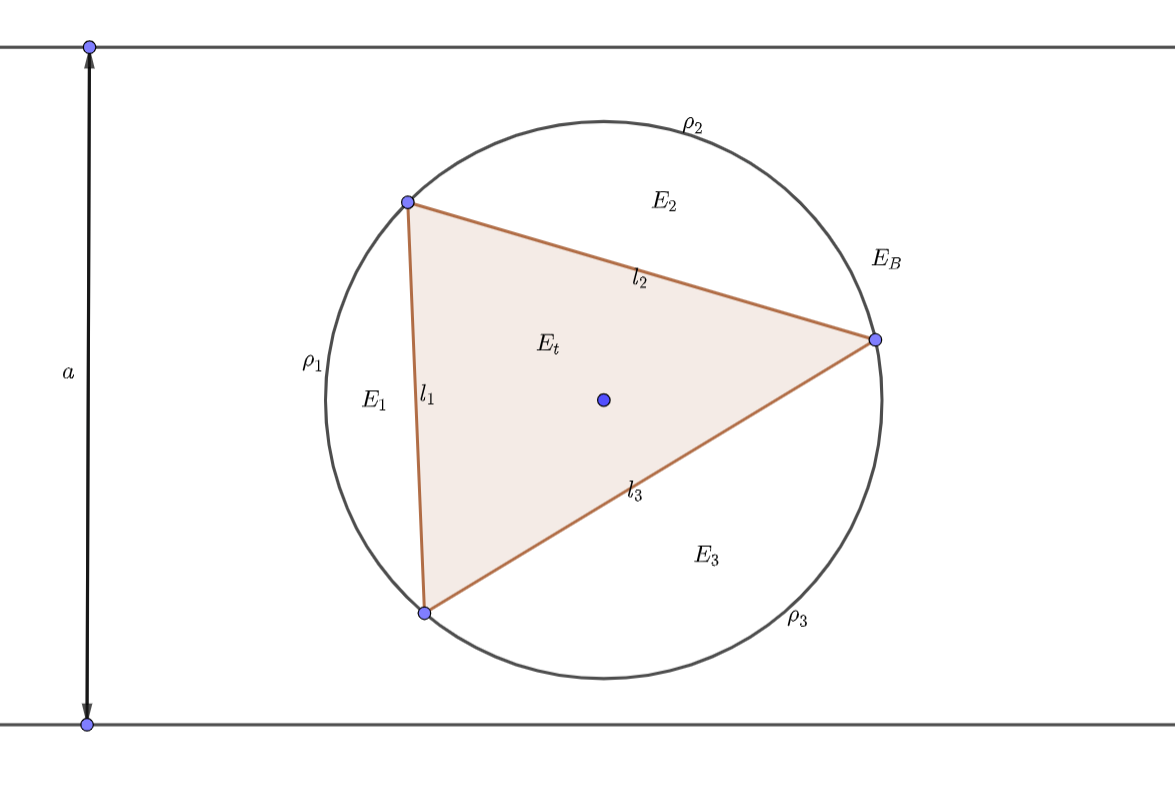
\includegraphics[width=0.8\textwidth]{figure.png}
}
% 表格模板
\renewcommand\arraystretch{0.8} % 设置表格高度为原来的0.8倍
\begin{table}[!htbp] % table标准
    \centering % 表格居中
    \begin{tabular}{p{1cm}<{\centering}p{1cm}<{\centering}p{3cm}<{\centering}p{5cm}<{\centering}} % 设置表格宽度
    %\begin{tabular}{cccc}
        \toprule
        $x_i$ & $f[x_1]$ & $f[x_i,x_{i+1}]$ & $f[x_i,x_{i+1},x_{i+2}]$ \\
        \midrule
        $x_0$ & $f(x_0)$ &                  &                          \\
        $x_0$ & $f(x_0)$ & $f'(x_0)$        &                          \\
        $x_0$ & $f(x_1)$ & $\frac{f(x_1)-f(x_0)}{x_1-x_0}$ & $\frac{f(x_1)-f(x_0)}{(x_1-x_0)^2}-\frac{f'(x_0)}{x_1-x_0}$\\
        \bottomrule
    \end{tabular}
\end{table}

\def\Log{\text{Log}} % 一个简单的宏定义
$\Log$ % 调用方法
\fi

\end{document}